\subsubsection{Neurale netværk}
Inden for machine learning findes et område kaldet deep learning. Deep learning går ud på at træne en algoritme til at træffe beslutninger, ud fra nogle såkaldte neurale netværk. Disse neurale netværk tager et eller flere inputs, og giver et output ud fra disse. 

Først vil vi kigge på den simpleste form for neuron i et neuralt netværk --- en perceptron\cite{neural}.
\begin{figure}[h!]
	\centering
	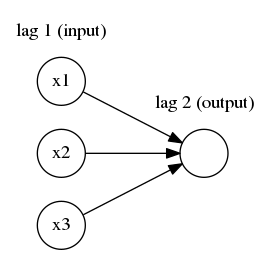
\includegraphics[width=0.3\textwidth]{images/neural1.png}
	\caption{Illustration af en perceptron}
	\label{fig:perceptron}
\end{figure}

En perceptron har \'et eller flere inputs, der alle kan være 0 eller 1. Vi tager udgangspunkt i figur \ref{fig:perceptron}, med 3 inputs. Alt efter de tre inputs til denne perceptron, vil outputtet enten være 0 eller 1. Vi indfører nu begrebet vægtning til netværket. Vægtningen består i at de forskellige inputs $x$ vægtes med et reelt tal $w$, og dermed betyder mere eller mindre end de andre inputs. Outputtet af perceptronen vil være $1$ hvis summen af alle vægte ganget med værdien af inputtet, er højere end en forudbestemt værdi.

\begin{figure}[h!]
	\centering
	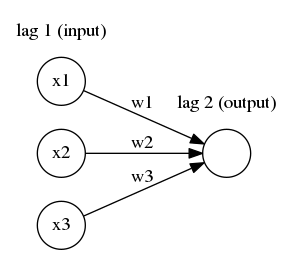
\includegraphics[width=0.3\textwidth]{images/neural2.png}
	\caption{Illustration af en perceptron med vægtning}
	\label{fig:perceptronWeight}
\end{figure}

Perceptroner giver enten outputtet 1 eller 0. Dette betyder at nogle små ændringer i inputtet eller vægtningen, kan betyde at outputtet går fra 0 til 1. For at undgå dette, bruger man en anden neuron, kaldet en sigmoid neuron. På samme måde som perceptronen, giver sigmoid også et output på baggrund af inputtet, men inputtet kan være et tal mellem 0 og 1, og outputtet vil også være et tal mellem 0 og 1. Outputtet af sigmoid neuronerne er givet ved sigmoid funktionen\cite{neural}.

\begin{equation}
	\sigma(z)=\frac{1}{1+e^{-z}}
\end{equation}
hvor $z=\vec{x}\cdot \vec{v} + b$, og $b$ er den negative værdi af den øvre grænse hvor en perceptron ville skifte mellem 0 og 1.

For at løse en given opgave ved hjælp af disse neuroner opstilles et `net' af neuroner, som består af inputs i første lag, outputtet i sidste lag og en række skjulte lag imellem. Når nettet er opstillet, kan det dog stadig være svært at vide hvilken vægt de forskellige inputs skal have, samt hvilke øvre grænser ($-b$) der skal bruges i funktionen ovenfor. Netværket er nemlig ikke trænet. Måden netværket trænes på er ved at opstille en \textit{cost-function}, som er en funktion som beskriver hvor godt outputtet passer overens med det faktiske resultat (supervised learning). Hvis cost-funktionen giver en højt resultat, ligger outputtet langt fra det rigtige svar, mens hvis resultatet er 0, har netværket ramt det rigtige svar. Ved at lave små justeringer på de forskellige vægte og øvre grænser, bliver netværket bedre og bedre til at få et lavet resultat fra cost-funktionen. Når netværket til sidst er trænet og kan svare rigtigt på alt træningsdata, kan det bruges til data uden for træningssættet, og stadig finde det rigtige resultat. 

Dagens og fremtidens selvkørende biler, benytter sig både af deep-learning teknikken samt semi-supervised learning\cite{Musk}. Både Tesla og Audi benytter sig af Nvidia Drive PX, hvilket er en udviklingsplatform, som tillader bilen det er installeret i, at tilgå Nvidias nye deep-learning platform kaldet DIGITS. Dette gør det muligt for enheder, at lære deres omgivelser at kende, og er designet til at fungere ligesom et menneske. Ligesom mennesker lærer med tiden og af deres erfaringer, vil bilerne også lære af deres erfaringer, men da de alle er koblet til dette netværk, lærer alle bilerne, af alle bilers erfaringer\cite{Nvidia}. Dette board uploader sine data til DIGITS, og hvis der er noget indsamlet data den ikke er sikker på hvad den skal gøre med, vil dette data blive kigget og regnet på af hele netværket.